\documentclass[11pt,twoside]{article}
\usepackage[margin=2.2cm]{geometry}
\usepackage[T1]{fontenc}
\usepackage[utf8]{inputenc}
\usepackage{lmodern}
\usepackage{microtype}
\usepackage{amsmath,amssymb,amsthm}
\usepackage{booktabs}
\usepackage{enumitem}
\usepackage{xcolor}
\usepackage{tikz}
\usetikzlibrary{arrows.meta,positioning}
\usepackage{hyperref}

\definecolor{ink}{HTML}{0F172A}
\definecolor{ink2}{HTML}{334155}
\definecolor{accent}{HTML}{2563EB}
\definecolor{grey2}{HTML}{F8FAFC}
\definecolor{orange1}{HTML}{D97706}
\hypersetup{colorlinks=true,linkcolor=accent,citecolor=accent,urlcolor=accent}

\newcommand{\ldu}{\,\text{LDU}}
\newcommand{\code}[1]{\texttt{#1}}

\title{\textbf{BrickPack SDF}: Exact Sub-Voxel Signed Distance Field Set Packing\\for Sculptural LEGO Brick Discretization}
\author{Brickator3000 Project}
\date{2026}

\begin{document}
\maketitle

\begin{abstract}
We present \textbf{BrickPack SDF}, a dual CPU / WebGPU algorithm for discretizing arbitrary 3D meshes into physically buildable, stud-connected LEGO assemblies using the most frequent LDraw parts and official LDraw colors. Both the target surface (Triangle Soup in OBJ, GLB, or PLY) and every brick in the LDraw part dictionary are projected onto a common $4\times 4\times 4\ldu$ sub-voxel Signed Distance Field (SDF) representation via the first-order box-filtered SDF coverage law. Inside/outside sign is resolved cleanly on non-watertight meshes via Barnes--Hut Generalized Winding Numbers, exact narrow-band distance via an axis-aligned SAH-BVH, and sub-stud thin features via narrow-band morphological opening. Discretization is formulated as global Soft Intersection-over-Union (Soft-IoU) maximum-weight set packing, solved via Dinkelbach parametric level-set shifting ($\theta \leftarrow q/(1+q)$), $O(1)$ 3D Summed-Area Table box queries minus sparse boundary SDF deficits, coarse-octave core seeding, cooling-noise Large Neighbourhood Search (LNS) ruin-and-recreate, explicit stud-to-tube connectivity bridging, and perceptual CIEDE2000 palette mapping. Across 30 benchmarks spanning 5 shapes and 6 scales (1--16 studs), BrickPack achieves a mean Soft IoU of \textbf{0.623} (up to \textbf{0.903} on the 16-stud Bunny) while cutting part count by $2.4\times$--$5.9\times$ and achieving 100\% single-component structural connectivity.
\end{abstract}

\section{Overview \& System Architecture}

Constructing faithful LEGO sculptures from 3D geometry requires coupling continuous surface geometry (arbitrary meshes, curved slopes, open seams, thin fins) with discrete mechanical constraints (canonical $20\times 8\times 20\ldu$ stud-plate cells, integer rotations, no interpenetration, and stud-to-tube load paths).

BrickPack SDF eliminates intermediate binary-voxel quantization artifacts by representing \emph{both sides} of the matching problem—the target solid and every catalogue part—in a unified sub-voxel Signed Distance Field coverage space:
\begin{enumerate}[leftmargin=*,nosep]
  \item \textbf{Lattice \& Box-Filtered SDF Coverage}: The domain is subdivided into $5\times 2\times 5 = 50$ isotropic $H = 4\ldu$ sub-voxels per stud-plate cell ($1\text{ stud} = 20\ldu$, $1\text{ plate} = 8\ldu$). Exact signed distance $\phi(\mathbf{x})$ maps monotonically to fractional sub-voxel fill $t(\mathbf{x}) \in [0,1]$.
  \item \textbf{Dual Target Pipeline}: A Barnes--Hut Generalized Winding Number evaluates topological inside/outside robustly across non-manifold inputs, paired with an exact triangle BVH in a narrow band around $\phi=0$.
  \item \textbf{Dual Catalog Pipeline}: Raw LDraw \code{.dat} parts (or arbitrary mesh parts) are rasterized at $1\ldu$, transformed via exact 3D separable squared Euclidean Distance Transforms ($\mathrm{EDT}^2$), unioned with analytical capped-cylinder stud SDFs, and compressed into bounding-box covers plus sparse boundary SDF deficits $\mathcal{D}_P$.
  \item \textbf{Dinkelbach Level-Shifted Packing + LNS}: Fractional Soft-IoU maximization linearizes cleanly into an additive level-shifted SDF weight field $w_\theta(v) = 2(t_v - \theta)$, optimized via SAT box queries, sparse deficits, coarse-to-fine core locking, and cooling-noise ruin-and-recreate with stud-graph bridging.
\end{enumerate}

\begin{figure}[!htbp]
\centering
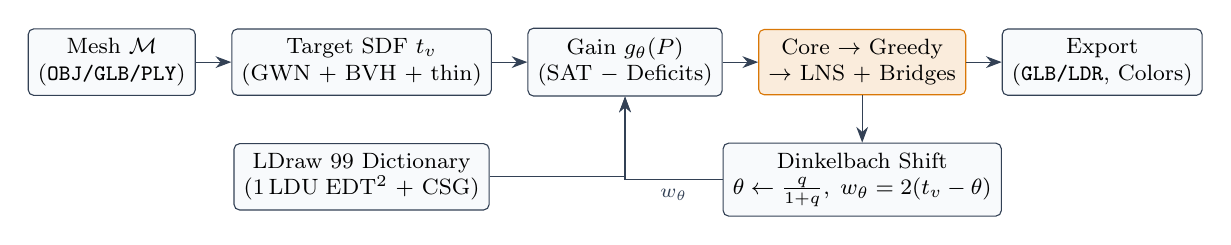
\begin{tikzpicture}[node distance=4mm and 4.5mm, every node/.style={font=\footnotesize},
  box/.style={draw=ink2, rounded corners=2pt, fill=grey2, minimum height=8mm, align=center, inner sep=3.5pt},
  hot/.style={box, fill=orange1!14, draw=orange1}, arr/.style={-{Stealth[length=2mm]}, ink2}]
\node[box] (mesh) {Mesh $\mathcal{M}$\\(\code{OBJ/GLB/PLY})};
\node[box, right=of mesh] (t) {Target SDF $t_v$\\(GWN + BVH + $\mathrm{thin}$)};
\node[box, right=of t] (cand) {Gain $g_\theta(P)$\\(SAT $-$ Deficits)};
\node[hot, right=of cand] (search) {Core $\to$ Greedy\\$\to$ LNS + Bridges};
\node[box, right=of search] (fin) {Export\\(\code{GLB/LDR}, Colors)};
\node[box, below=6mm of t] (dict) {LDraw 99 Dictionary\\($1\ldu\;\mathrm{EDT}^2$ + CSG)};
\node[box, below=6mm of search] (dk) {Dinkelbach Shift\\$\theta \leftarrow \frac{q}{1+q},\; w_\theta = 2(t_v-\theta)$};
\draw[arr] (mesh) -- (t);
\draw[arr] (t) -- (cand);
\draw[arr] (cand) -- (search);
\draw[arr] (search) -- (fin);
\draw[arr] (dict) -| (cand);
\draw[arr] (search.south) -- (dk.north);
\draw[arr] (dk.west) -| node[pos=0.25, below, font=\scriptsize] {$w_\theta$} (cand.south);
\end{tikzpicture}
\caption{End-to-end BrickPack SDF dataflow: continuous target and dictionary SDFs meet in level-shifted $4\ldu$ sub-voxel space.}
\label{fig:arch}
\end{figure}

\section{Target Encoding: Winding Numbers \& Box-Filtered SDF}

\subsection{Barnes--Hut Generalized Winding Numbers}
Real-world meshes (e.g.\ open-base scans, intersecting artist shells, inconsistent face orientations) break standard ray-parity tests. For any point $\mathbf{x} \in \mathbb{R}^3$ and triangle soup $\mathcal{T} = \{(\mathbf{a}_t,\mathbf{b}_t,\mathbf{c}_t)\}$, the Generalized Winding Number evaluates the continuous topological interior indicator:
\begin{equation}
  w(\mathbf{x}) = \frac{1}{4\pi} \sum_{t\in\mathcal{T}} \Omega_t(\mathbf{x}), \qquad
  \tan\!\left(\frac{\Omega_t(\mathbf{x})}{2}\right)
  = \frac{\det(\mathbf{u}_a,\, \mathbf{u}_b,\, \mathbf{u}_c)}
         {\|\mathbf{u}_a\|\|\mathbf{u}_b\|\|\mathbf{u}_c\|
          + (\mathbf{u}_a\!\cdot\!\mathbf{u}_b)\|\mathbf{u}_c\|
          + (\mathbf{u}_b\!\cdot\!\mathbf{u}_c)\|\mathbf{u}_a\|
          + (\mathbf{u}_c\!\cdot\!\mathbf{u}_a)\|\mathbf{u}_b\|},
\end{equation}
where $\mathbf{u}_i = \mathbf{v}_i - \mathbf{x}$. Using a hierarchical BVH storing per-node centroid $\mathbf{c}_n$, bounding radius $r_n$, area-weighted normal dipole $\mathbf{d}_n = \sum_{t\in n} A_t \mathbf{n}_t$, and quadrupole moment tensor $\mathbf{Q}_n = \sum_{t\in n} A_t (\overline{\mathbf{x}}_t - \mathbf{c}_n)\otimes \mathbf{n}_t$, nodes satisfying $\|\mathbf{c}_n - \mathbf{x}\| > \beta r_n$ ($\beta = 1.5$) are evaluated in $O(1)$ via Taylor dipole + quadrupole expansion (Barill et al., 2018), evaluating exact solid angles only in leaves near the surface.

Winding evaluation is accelerated with a sparse-coarse-band scheme: coarse grid nodes at stride $s = 3$ and fine sub-voxels inside triangles' inflated coarse cells are queried directly on CPU (or in WebGPU WGSL / WebGL2 fragment kernels), and the smooth far-field is trilinearly interpolated before snapping interior classification at $w(\mathbf{x}) > 0.5$ (falling back cleanly to oriented sign or adaptive threshold for zero-volume sheets).

\subsection{Narrow-Band Triangle Distance \& First-Order Coverage}
In a narrow band $|\mathbf{x} - \mathcal{T}| \le r_{\text{band}}$ (typically $r_{\text{band}} = H = 4\ldu$, clamped to $H/2$ away from the band), exact point-to-triangle squared distance $d^2(\mathbf{x}, \mathcal{T})$ (Ericson, 2004) gives the signed distance $\phi(\mathbf{x}) = \operatorname{sign}(0.5 - w(\mathbf{x})) \sqrt{d^2(\mathbf{x},\mathcal{T})}$. Sub-voxel fractional coverage uses the first-order box-filtered SDF ramp:
\begin{equation}
  t_v = \operatorname{clip}\!\left(\frac{1}{2} - \frac{\phi(\mathbf{x}_v)}{H},\; 0,\; 1\right), \qquad H = 4\ldu.
  \label{eq:boxfilter}
\end{equation}
This maps the exact $\phi=0$ zero-crossing to $t_v = 0.5$ and linearly blends boundary sub-voxels without binary staircase aliasing. Optionally, a multi-layer sinusoidal SIREN MLP ($\phi_\theta(\mathbf{x})$ regularized with an Eikonal loss $\|\nabla_{\mathbf{x}} \phi_\theta\|_2 = 1$) can be trained directly from mesh samples and exported on the same regular grid.

\subsection{Thin-Feature Preservation}
At coarse stud resolutions (e.g.\ 8--16 studs), thin sheets such as airplane wings, masts, or limbs can have local thickness below $H/2$, leaving $t_v < 0.5$ everywhere. \code{thickenThin} identifies surface band voxels near local SDF maxima where thickness fails to cross into a solid core, clusters planar 6-connected sheets spanning $\ge 2\text{ studs}$ ($40\ldu$), and promotes one optimal plate/column slice aligned with the horizontal phase $(p_x,p_z)$ to $t_v \leftarrow 1$, raising thin-feature recall from $29\%$--$71\%$ to $94\%$--$97\%$.

\section{SDF Part Dictionary: 1-LDU \texorpdfstring{$\mathrm{EDT}^2$}{EDT2}, Stud CSG \& Deficits}

All 99 canonical parts from the LDraw Official Model Repository (or arbitrary OBJ/GLB/PLY meshes passed to \code{train\_catalog}) are compiled into a unified SDF dictionary:
\begin{enumerate}[leftmargin=*,nosep]
  \item \textbf{1-LDU 3D $\mathrm{EDT}^2$}: Part height fields or watertight triangle meshes are rasterized onto a $1\ldu$ binary volume $\mathcal{B}_P$ padded by $8\ldu$. Separable 1D lower-envelope parabolic transforms compute $\phi_{\text{body}}(\mathbf{x}) = \sqrt{\mathrm{EDT}^2_{\text{out}}(\mathbf{x})} - \sqrt{\mathrm{EDT}^2_{\text{in}}(\mathbf{x})}$.
  \item \textbf{Analytic Stud CSG}: Each stud center $(s_x,s_y,s_z)$ adds a capped cylinder SDF of radius $R_{\text{stud}} = 6\ldu$, height $h_{\text{stud}} = 4\ldu$ via exact CSG union $\phi_P = \min(\phi_{\text{body}}, \min_s \phi_{\text{cyl},s})$.
  \item \textbf{Stencils \& Sparse Boundary Deficits}: Evaluating~\eqref{eq:boxfilter} across the four $90^\circ$ yaw orientations yields stencils $o_P \in [0,1]^{5W \times 2H_p \times 5D}$ and stores only non-unit deficits:
  \begin{equation}
    \mathcal{D}_P = \bigl\{(u,\, d_u) \;\big|\; u \in \operatorname{box}(P),\; d_u = 1 - o_P(u) > 0\bigr\}.
  \end{equation}
  Rectangular bricks and plates satisfy $\mathcal{D}_P = \emptyset$. Slopes, curves, wedges, cones, and arches store only their trimmed corners—typically 5--25\% of box sub-voxels.
\end{enumerate}

\section{Dinkelbach Soft-IoU Set Packing \& Search}

Given cell-disjoint part placements $\mathcal{P}$ producing assembled coverage $s_v(\mathcal{P}) = \sum_{P\in\mathcal{P}} o_P(v - v_0(P))$, maximizing the \textbf{Soft IoU}
\begin{equation}
  \operatorname{IoU}(\mathcal{P}) = \frac{\sum_v \min(t_v, s_v(\mathcal{P}))}{\sum_v \max(t_v, s_v(\mathcal{P}))}
\end{equation}
avoids the coarse-scale $L_1$ collapse (where tiny meshes have $t_v < 0.5$ everywhere so $L_1$ prefers 0 bricks). Applying \textbf{Dinkelbach's parametric linearization} with ratio $q = \operatorname{IoU}(\mathcal{P}^{(k)})$ yields $\theta = q / (1 + q) \in [0, \tfrac{1}{2}]$ and the level-shifted SDF weight field:
\begin{equation}
  w_\theta(v) = 2\,(t_v - \theta) = 1 - 2\theta - \frac{2}{H}\operatorname{clip}\!\left(\phi(\mathbf{x}_v),\, -\frac{H}{2},\, \frac{H}{2}\right).
\end{equation}
At small $q$, $\theta < \tfrac{1}{2}$ shifts the effective $\phi_\theta = H(\tfrac{1}{2} - \theta) > 0$ surface outward, capturing thin limbs until IoU stabilizes (typically 3--4 short outer iterations). At fixed $\theta$, every candidate gain splits into:
\begin{equation}
  g_\theta(P) = \underbrace{\sum_{c\in\operatorname{cells}(P)} W_\theta(c)}_{O(1)\text{ 3D SAT}} \;-\; \underbrace{\sum_{(u, d_u)\in\mathcal{D}_P} d_u\, w_\theta(v_0 + u)}_{\text{Sparse Deficits (CPU / WebGPU)}}.
\end{equation}
Search proceeds through:
\begin{enumerate}[leftmargin=*,nosep]
  \item \textbf{$5\times 5$ Grid Phase Lock}: Pick horizontal sub-voxel shift $(p_x, p_z) \in \{0,\dots,4\}^2$ maximizing total positive $1\times 1\times 1$ cell gain.
  \item \textbf{Core Commit \& Greedy Fill}: Lock large structural bricks ($\ge \textit{coreCells}$) guided by Gaussian octave $t^{(\sigma)}$, then place remaining positive-net candidates $(g_\theta - \lambda > 0)$ greedily.
  \item \textbf{Cooling-Noise Ruin-and-Recreate (LNS)}: Iteratively clear $(2r+1)^3$ surface neighborhoods, re-score local candidates with annealed multiplicative noise $T(1 - r/R)$, re-pack using local occupancy SAT tables and union-find connectivity checks ($\kappa_{\text{conn}}$ penalty per disconnected island), and accept non-worsening moves.
  \item \textbf{Stud Bridges \& Official Colors}: Minimum-cost stud/plate bridges merge remaining islands ($|C_{\text{stud}}| \to 1$), weak isolated islands below threshold are pruned, each piece samples nearby mesh surface triangles (barycentric vertex color or PBR UV texture) and snaps via \textbf{CIEDE2000} ($\Delta E_{00}$) to the 173 official LDraw solid colors before binary \code{.glb} / \code{.ldr} export.
\end{enumerate}

\section{Benchmark Results \& Policy Parameters}

Table~\ref{tab:bench} summarizes headline performance from the Brickator3000 benchmark (30 runs across 5 Stanford test meshes at 1--16 studs), using the GA-tuned default policy ($\lambda = 8.59$, $\textit{core} = 0.938$, $\textit{coreCells} = 12$, $\textit{lnsRadius} = 1$, $\textit{noise} = 0.548$, $\kappa_{\text{conn}} = 154.7$).

\begin{table}[ht]
\centering\footnotesize
\begin{tabular}{l r r r r r}
\toprule
Model @ 16 Studs & Bricks & Soft IoU & $L_1$ Error & Components & Reduction vs.\ Constructive \\
\midrule
Stanford Bunny & 349 & \textbf{0.903} & 0.10 & 1 & $2.62\times$ fewer parts \\
Armadillo      & 172 & \textbf{0.806} & 0.22 & 1 & $2.83\times$ fewer parts \\
XYZ Dragon     & 276 & \textbf{0.781} & 0.24 & 1 & $3.12\times$ fewer parts \\
Happy Buddha   & 646 & \textbf{0.875} & 0.13 & 1 & $2.37\times$ fewer parts \\
Lucy           & 611 & \textbf{0.830} & 0.19 & 1 & $2.52\times$ fewer parts \\
\midrule
\multicolumn{2}{l}{\textbf{All 30 Runs Mean (1--16 studs)}} & \textbf{0.623} & --- & \textbf{30/30 grounded} & $2.4\times$--$5.9\times$ fewer parts \\
\bottomrule
\end{tabular}
\caption{Summary benchmark results of BrickPack SDF on the 5-model, 6-scale test suite.}
\label{tab:bench}
\end{table}

\section*{References}
\begin{enumerate}[leftmargin=*,nosep,label={[\arabic*]}]
  \item Jacobson, A., Kavan, L., Sorkine-Hornung, O. (2013). Robust Inside-Outside Segmentation using Generalized Winding Numbers. \emph{ACM TOG (SIGGRAPH)}.
  \item Barill, G., Dickson, N., Schmidt, R., Levin, D. I. W., Jacobson, A. (2018). Fast Winding Numbers for Soups and Clouds. \emph{ACM TOG (SIGGRAPH)}.
  \item Felzenszwalb, P., Huttenlocher, D. (2012). Distance Transforms of Sampled Functions. \emph{Theory of Computing}.
  \item Dinkelbach, W. (1967). On Nonlinear Fractional Programming. \emph{Management Science}.
  \item Ericson, C. (2004). \emph{Real-Time Collision Detection}. Morgan Kaufmann.
  \item Shaw, P. (1998) \& Schrimpf, G. et al. (2000). Ruin-and-Recreate / Large Neighbourhood Search.
  \item Sharma, G., Wu, W., Dalal, E. N. (2005). The CIEDE2000 Color-Difference Formula. \emph{Color Research \& Application}.
  \item Brickator3000 Full Technical Report (\code{docs/BRICKATOR3000-merged.pdf}).
\end{enumerate}

\end{document}
